\documentclass{article}[12pt]
%\usepackage{fullpage}
%\usepackage{fullpage}
\usepackage{amsmath}
\usepackage{latexsym}
\usepackage{amssymb,amsfonts}
\usepackage{graphicx}
\usepackage{graphics}
\usepackage[margin=.75in]{geometry}

\graphicspath{ {../../images/} }

\begin{document}

\newcommand{\activityname}{
  Math Abridged
}
\newcommand{\subtitle}{
  An Optimal Optimization Puzzle
}

\phantom{.}\hspace{-.5in}\begin{tabular}{lr}
 \begin{tabular}{l}
    
\includegraphics[width=2in]{AUExploreLogo.pdf}
 \end{tabular}
 & \hspace{.5in}
 \begin{tabular}{r}
    {\Huge \activityname}
 \end{tabular}
\end{tabular}
\thispagestyle{empty}

\noindent\hrulefill
\phantom{.}\vspace{.15in}

Trapped in the frightning country of \textbf{Badlandia}, your brave group of four adventurers has almost escaped to the lush hills of \textbf{Nicetopia}. All that remains is one dark, rickity bridge...

\begin{figure}[h]
\begin{center}
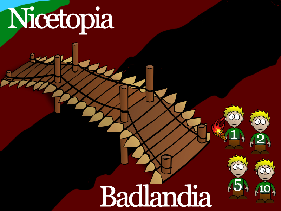
\includegraphics[width=3in]{bridge.pdf}
\end{center}
\end{figure}

As you plan your escape, the earth begins to tremble. An \textbf{earthquake} is coming, and you only have minutes to spare before the bridge \textbf{collapses}!

\begin{itemize}
\item Each person crosses the bridge at different speeds: \textbf{1 minute, 2 minutes, 5 minutes, or 10 minutes}.
\item You have one torch, which only has enough light for \textbf{at most two people crossing the bridge at a time}.
\item If two people cross the bridge at the same time, the both move at the same speed as the \textbf{slower} adventurer, so they can share the torch.
\end{itemize}

You don't know how much time you have - can you get your group across the bridge in the fastest time possible?!


\end{document}
